\documentclass[12pt]{article}
\usepackage[T2A]{fontenc}
\usepackage[utf8]{inputenc}
\usepackage[english,russian]{babel}
\usepackage{amssymb,amsmath,amsthm, mathtools}
\usepackage{subfigure}
\newcommand\independent{\protect\mathpalette{\protect\independenT}{\perp}}
\DeclareMathOperator{\trace}{trace}
\def\independenT#1#2{\mathrel{\rlap{$#1#2$}\mkern2mu{#1#2}}}


\newtheorem{note}{Замечание}
\newtheorem{theorem}{Теорема}
\newtheorem{dfn}{Определение}
\newtheorem{utv}{Утверждение}
\newtheorem{example}{Пример}

\begin{document}
\section{Введение, мотивация}
Рассмотрим следующую задачу:
Предположим, что имеется некоторое изображение (ддя простоты бинарное -- пусть каждый пиксель либо белый цвет, либо черный), а потом пришел кто-то вредный и случайно переключил некоторые пиксели с черного на белый и наоборот. 

Задача -- восстановить исходное изображение (избавиться от шума). 

Мы можем представить все это следующим графом, представленным на рисунке \ref{fig:ex}. $Y_i$ --- это те пиксели, которые мы видим (зашумленные), $X_i$ --- исходные пиксели. При этом, каждый $X_i$ и $Y_i$ принимает значение в множестве $\{ -1; +1\}$. (-1 -- черный цвет, +1 -- белый).
Заметим, что каждый $Y_i$ -- связан ребром только с $X_i$, а каждый $X_i$ связан ребрами только с соседними.


\textbf{Пояснение}: это вполне логично, потому что зашумленный пиксель связан по сути только с исходным пикселем. А связь соседних исходных $X_i$ друг с другом обусловлена тем, что <<в реальном мире>> на изображениях соседние пиксели как правило находятся в одном и том же состоянии (либо оба белые, либо оба черные).
\begin{figure}[hhh]
\centering
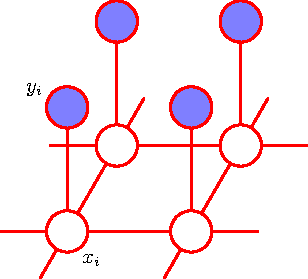
\includegraphics[width=.5\linewidth]{./figures/image.pdf}
\label{fig:ex}
\caption{Image denosing}
\end{figure}

Таким образом, если мы будем считать, что $X_i$, $Y_i$ --- это случайные величины (имеющие распределение Бернулли), а ребра между ними указывают на связи этих случайных величин, то мы и получим определение случайного поля. 

Теперь опишем это формально:

\section{Формальное определение марковского поля (МП), скрытого марковского поля (СМП)}
Пусть $A = \{ 1, 2, \ldots, a\}$ и $B = \{1, 2,\ldots b\}$, $a, b < \infty$ --- два конечных
множества. Пусть $S = \{1, 2,  \ldots,  N\}$ --- конечное множество индексов.
Пусть $X = \{X_i \mid i \in S\}$ — многомерная случайная величина, такая что каждая компонента $X_j$ , являющаяся одномерной случайной величиной, принимает значение $x_j$ и определена в своем вероятностном пространстве. Считается, что $\forall j \ X_j$ дискретны (хотя могут быть и непрерывны), определены на одном
вероятностном пространстве и множество значений — конечно.
Для удобства рассмотрения можно представлять, что множество
индексов $S$ задает множество точек на плоскости. Соответственно, рассматривается реализация многомерной случайной величины $X$ в этих точках. Введенная таким образом случайная величина $X$ называется случайным полем.

Конкретная реализация $x = (x_1, \ldots, x_N)$ многомерной случайной величины $X$, то есть совместное событие $(X_1 = x_1, \ldots, X_N = x_N)$ (кратко $X = x$), называется конфигурацией $X$. Пусть X --- случайное поле со значениями на множестве A, то есть $\forall i  \ X_i \in A$. Если $x$ --- какая-то конкретная конфигурация $X$, то $\mathcal{X}$ ---
множество всех возможных конфигураций:
\begin{gather*}
\mathcal{X} = \{ x = (x_1, \ldots, x_N) \mid x_i \in A \forall i \in S\}.
\end{gather*}
Система соседства --- это множество $\partial = \{\partial i\mid i \in S \}$, где $\partial i$ --- множество элементов из $S $, называемое шаблоном соседства для элемента $i$, такое что:
\begin{gather*}
\begin{cases}
i \not \in \partial i, \\
i \in \partial j \Leftrightarrow j \in \partial i
\end{cases}
\end{gather*}

\begin{dfn}
Случайное поле $X$ называется марковским случайным полем в соответствии с системой соседства $\partial$ тогда
и только тогда, когда $\forall i$:

\begin{gather*}
\begin{cases}
P(X = x) > 0 \ \forall x \in \mathcal{X}, \\
p(X_i = x_i \mid X_j = x_j, j \in S \setminus \{i\}) = P(X_i = x_i \mid X_j = x_j, j \in \partial i),
\end{cases}
\end{gather*}
\end{dfn}

\textbf{Пояснение}: по сути это определение означает, что распределение случайной величины в конкретной вершине зависит только от соседних случайных величин (то есть от тех, что соединены с ней ребром). А это свойство и есть в каком-то смысле <<марковское>>.


\begin{dfn}
Скрытое марковское случайное поле --- пара случайный полей $(X, Y)$, такая что 
\begin{enumerate}
\item $X = \{ X_i \mid i \in S \}$ --- так называемое <<скрытое>> (или, другими словами, ненаблюдаемое) марковское поле со значениями в $A$.
\item  $Y = \{ Y_i \mid i \in S \}$  наблюдаемое (вовсе не обязательно марковское) случайное поле со значениями в $B$. Важно, что $\forall j \in S, \forall d \in A$,известны условные распределения $P(Y_i \mid X_i = d)$.
\item Для любой конфигурации $x\in \mathcal{X}$ случайные величины $Y_i$ условно независимы, то есть
\begin{gather*}
P(Y\mid X = x) = \prod\limits_{i \in S} P(Y_i\mid X_i = x_i).
\end{gather*}
\end{enumerate}
\end{dfn}
Скрытое марковское случайное поле можно себе представлять как
наблюдаемое случайное поле $Y$, каждой точке которого соответствует ненаблюдаемое (скрытое) марковское случайное поле $X$. 

\textbf{Пояснение}: Возвращаемся к примеру с очисткой изображения от шума -- там случайное поле было скрытым (наблюдались только зашумленные состояния).


\section{Задачи, связанные с МП/СМП}
По сути МП -- это удобный язык, описывающий вероятностные модели. В связи с этим, возникает несколько стандартных задач. 
\begin{enumerate}
\item Оценка параметров совместного распределения случайных величин (о том, как определяется совместное распределения для МП будет сказано позже)
\item Мы знаем параметры модели и хотим считать например самую вероятную конфигурацию (ну или вероятность каждой конфигурации в более общем смысле) (как в примере про очистку шума -- самый вероятный набор $X_i$ будет <<изображением без шума>>)
\end{enumerate}

Стоит еще отметить, что нам хочется описать задачу такой МП, чтобы у нее мало ребер. Почему? 
Рассмотрим полный граф (т.е. граф у которого все вершины соединены ребрами между собой) и представим, что случайная величина в каждой вершине имеет дискретное распределение на множестве $\{ 1, \ldots, K \}$. Если таких вершин $n$, то всего надо оценить $k^n - 1$ параметров, что очень грустно. 
\begin{figure}[h!]
\centering
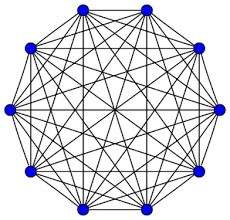
\includegraphics[width=.3\linewidth]{./figures/full.png}
\label{fig:hmm}
\caption{Пример полного графа}
\end{figure}


\section{Про совместное распределение}

\begin{dfn}
Клика $c$ для системы соседства $\partial$ --- множество элементов из $S$,  такое что $\forall s, r \in c, s \ne r \Rightarrow r \in \partial s$. Несложно заметить,
что любое подмножество клики --- также клика (считается, что любое одноэлементное множество также является кликой; в этом случае такая клика называется тривиальной). 
\end{dfn}
Пример клик можно видеть на рисунке \ref{fig:cliques}.

\begin{figure}[hh]
\centering
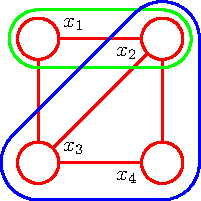
\includegraphics[width=.3\linewidth]{./figures/cliques.pdf}
\label{fig:cliques}
\caption{Клики}
\end{figure}

Пусть $c$ --- клика, а $x_c$ --- ограничение конфигурации $x$ на $c$, то есть $x_c = (x_{i_1}, x_{i_2}, \ldots x_{i_{|c|}})$, где $i_j \in c, j = 1, \ldots, |c|$. Пусть $C(\partial)$ --- множество всех клик для системы соседства $\partial$, тогда потенциальная функция $V_c(x_c)$ определяется как любая функция $V : C(\partial) \rightarrow R$.


\begin{dfn}
Дискретное распределение называется распределением Гиббса, если
\begin{gather}
P(X=x) = \frac1Z \exp \left( - \sum\limits_{x\in C(\partial)} V_c(x_c) \right), 
\label{eqn:distr}
\end{gather}
где $Z$ --- нормирующая константа, такая что:
\begin{gather}
Z = \sum\limits_{x\in \mathcal{X}} \exp \left( - \sum\limits_{x\in C(\partial)} V_c(x_c)  \right).
\label{eqn:const}
\end{gather}
\end{dfn}
Очевидно, что в случае нулевых потенциальных функций для какого-нибудь набора клик, соответствующие члены будут просто отсутствовать в формулах \eqref{eqn:distr}, \eqref{eqn:const}.
Наиболее важной теоремой, связывающей марковские случайные
поля и распределение Гиббса, является следующая
\begin{theorem}[Hammersley-Clifford]
$X$ --- марковское случайное поле тогда и только тогда, когда $P(X = x)$--- распределение Гиббса.
\end{theorem}

\textbf{Пояснение}: данная теорема дает полное описание совместного распределения для любой МП. Таким образом, распределение распадается в сумму распределений по каждой клике.

\begin{example}
В нашем примере очистки изображения от шума (рисунок \ref{fig:ex}) совместное распределение будет иметь вид
\begin{gather*}
p(x, y) = -\frac{1}{Z} \exp\{ -E(x, y)\}, \\ 
E(x, y) = \alpha \sum\limits_i x_i - \beta \sum\limits_{ \{i, j \} } x_i x_j -   \\ \gamma \sum\limits_{ \{i, j \} } x_i y_j
\end{gather*}
Во-первых, видно, что это распределение -- распределение Гиббса.
Параметh $\beta$ -- это параметр зависимости соседних $x_i$, $\alpha$ -- вклад каждого $x_i$ отдельно, $\gamma$ отвечает за взаимосвязь скрытого и наблюдаемого пикселя.
\end{example}

\newpage
\section{Скрытые марковские модели}
Частным случаем СМП является скрытая марковская модель, формальное определение ниже
\begin{dfn}
Скрытая марковская модель --- это дважды случайный процесс, то есть модель, состоящая из $N$ состояний,
в каждом из которых некоторая система может принимать одно из
$M$ значений какого-либо параметра. Вероятности переходов между
состояниями задаются матрицей вероятностей $A = (a_{ij})$, где $a_{ij}$ — вероятность перехода из $i$-го в $j$-е состояние. Вероятности выпадения каждого из $M$ значений параметра в каждом из $N$ состояний
задаются матрицей $B = (b_{jk})$, где $b_{jk}$ — вероятность выпадения $k$-го
значения параметра в $j$-м состоянии. Вероятность наступления начального состояния задается вектором $\pi = (\pi_i)$ , где $\pi_i$ --- вероятность
того, что в начальный момент система окажется в $i$-м состоянии.
\end{dfn}

Полагается, что наблюдаемые значения $Y_k$ зависят только от соответствующего им скрытого состояния марковской цепи $X_j$, то есть $P(Y = y \mid X = x) = \prod\limits_{i = 0}^{n} P(Y_i = y_i \mid X_i = x_i)$. Таким образом, скрытой
марковской моделью называется тройка $\lambda = (A, B, \pi)$.

Возьмем скрытую марковскую модель, функционирующую в дискретном времени. Пусть при некотором ее функционировании при проходе через состояния $x_0, \ldots, x_n$ на выход подавались буквы $y_0, \ldots, y_n$ соответственно. Рассмотрим многомерную случайную
величину
\begin{gather*}
Z = (Z_1, \ldots, Z_{2n + 2}) = (X_0, Y_0, \ldots, X_n, Y_n),
\end{gather*}
причем вероятность $P(X_i = x_i \mid X_{i-1} = x_{i-1})$ --- это вероятность перехода $a(x_{i-1}, x_{i})$ из состояния $x_{i-1}$ в состояние $x_i$, а вероятность $P(Y_i  = y_i \mid X_i = x_i)$ это вероятность $b(y_i, x_i)$ выдачи буквы $y_i$ в состоянии $x_i$. Назовем такую многомерную случайную величину скрытой порожденной случайной величиной.


\begin{utv}
Любая скрытая порожденная случайная величина — это случайное марковское поле специального вида (см. рис. \ref{fig:hmm}).
\end{utv}
\section{Алгоритм Витерби}
На примере скрытой марковской цепи опишем алгоритм Витерби (существует его обобщение на скрытые марковские поля).
Данный алгоритм вычисляет наиболее вероятную последовательность скрытых состояний $X_i$, при условии наблюдаемой последовательности состояний $Y_i$. 

Наиболее вероятная последовательность состояний $x_1, \ldots, x_n$ будет вычисляться при помощи следующих рекуррентных соотношений
\begin{itemize}
\item $\phi_{1,k} = b_{1,k} \cdot \pi_k$
\item $\phi_{\ell,k} = b_{\ell,k} \cdot \max\limits_{i \in S} (a_{i, k} \cdot \phi_{\ell-1, i})$.
\end{itemize}
Здесь $\phi_{\ell, k}$ — это вероятность наиболее вероятной последовательности состояний, ответственная за появление первых $\ell$ наблюдаемых символов, завершающаяся в состоянии $k$.
Иными словами, если мы наблюдаем состояние $y_1$, то вероятность делится на следующие вероятности:
\begin{enumerate}
\item Получить скрытое состяние <<1>> с вероятностью $\pi_1$ и получить наблюдаемое состояние $y_1$ с вероятностью $b_{1,1}$.
\item Получить скрытое состяние <<2>> с вероятностью $\pi_2$ и получить наблюдаемое состояние $y_1$ с вероятностью $b_{2,1}$.
\item \ldots
\end{enumerate}

\end{document}